\section{The Rodin Platform}
\label{reference_01}

This Chapter should give the user an overview about the UI elements he might encounter.

\subsection{Eclipse in General}

Just references to other resources.

\subsection{The Event-B Perspective}

\marginpar{The Event-B perspective: We briefly describe the various views (Event-B explorer, structure editor, outline view, symbol view) and their content. We want to cover every element of each view (like buttons, entry fields, etc.), but for the underlying theory we link to the other reference sections. The relevant menu entries are also described.}

Figure \ref{fig_ref_01_eventb_perspective1} shows an overview of the initial situation of the Event-B Perspective. The following subsections name the different Rodin GUI elements (i.e. Views) which are visible and explain their functions.

\imagedpi{img/reference/ref_01_eventb_perspective1.pdf}{150mm}{img/reference/ref_01_eventb_perspective1.png}{Overview of the Event-B Perspective}{fig_ref_01_eventb_perspective1}

\subsubsection{Menu bar}

The menu bar of provides for instance file and edit operations.

\subsubsection{Tool bar}

The tool bar provides short cuts for familiar commands like save, print, undo and redo. Furthermore, the tool bar provides wizard short cuts for creating elements like axioms, constants, enumerated sets, etc. which are described in section \ref{ref_01_the_eventb_editor}.

\subsubsection{Editor View}

The editor view contains the active Event-B editor which is described in section \ref{ref_01_the_eventb_editor}.

\subsubsection{Outline View}

The outline view displays the outline of the active Event-B editor, and lists elements like axioms, variables, etc.. 

\subsubsection{Rodin Problems View}

he Rodin Problems view shows problems (i.e. syntax errors) of the active Event-B editor.

\subsubsection{Symbols View}
\label{reference_01_symbols_view}

The symbols view is intended to give users a convenient way to type in mathematical symbols into the various model editors. If an editor is open and a text field is active (the cursor is blinking), then clicking a symbol inserts it at the current position as demonstrated in figure \ref{fig_ref_01_symbol_table1}. 

The ASCII code corresponding to the symbol where the mouse hovers is also displayed as a tooltip, so that the user can also learn how to input symbols directly. 

\begin{figure}[!h]
\begin{center}
	\includegraphics{img/reference/ref_01_symbol_table1.png}
	\caption{Clicking a symbol inserts it at the current position}
	\label{fig_ref_01_symbol_table1}
\end{center}
\end{figure}

\subsubsection{Event-B Explorer}
\label{reference_01_eventb_explorer}

Projects are reachable in the RODIN platform by means of a view called the \textsf{Event-B Explorer}. This view is usually situated on the left hand side of the screen as shown in figure \ref{fig_ref_01_eventb_perspective1}. The \textsf{Event-B Explorer} contains a list of name of the current projects. Next to each project name is a little triangle. By pressing it, one can expand a project and see its components like machines and contexts.

The icons (\icon{rodin/ctx_obj.png} or \icon{rodin/mch_obj.png}) situated next to the components help recognizing their kind (context or machine respectively).

In expanding a machine (respectively a context), you can explore its elements. Double clicking on a specific element (i.e. a variable) opens the Event-B editor and marks the position of the variable in the machine (respectively in the context) as shown in figure \ref{fig_ref_01_project_explorer1}. Furthermore, proof obligations are displayed at tree structure's leafs (for more information see section \ref{ref_01_proving_perspective}).

\begin{figure}[!h]
\begin{center}
	\includegraphics{img/reference/ref_01_project_explorer1.png}
	\caption{Double clicking on an element opens the Event-B editor and marks the corresponding position}
	\label{fig_ref_01_project_explorer1}
\end{center}
\end{figure}

\subsection{The Event-B Editor}
\label{ref_01_the_eventb_editor}

Once a context (or respectively a machine) is created, a window appears in the editing area as shown in figure \ref{fig_ref_01_eventb_editor1}.

\begin{figure}[!h]
\begin{center}
	\includegraphics{img/reference/ref_01_eventb_editor1.png}
	\caption{The Event-B editor}
	\label{fig_ref_01_eventb_editor1}
\end{center}
\end{figure}

You are in the "Edit" area allowing you to edit modelling elements of the context, namely dependencies (keyword "EXTENDS"), carrier sets (keyword "SETS"), constants (keyword "CONSTANTS"), or axioms (keyword "AXIOMS"). By pressing the triangle (\icon{rodin/collapsed.png}) next to each keyword, you can add, remove, or move corresponding modelling elements. As an example, figure \ref{fig_ref_01_eventb_editor2} shows what you obtain after pressing the triangle next to the keyword "AXIOMS".

\begin{figure}[!h]
\begin{center}
	\includegraphics{img/reference/ref_01_eventb_editor2.png}
	\caption{By pressing the triangle you can collapse/expand context sections}
	\label{fig_ref_01_eventb_editor2}
\end{center}
\end{figure}

By pressing the \icon{rodin/add.png} button, you can add a new modelling element. For instance clicking on the \icon{rodin/add.png} button next in the "AXIOMS" section will add a new axiom element. You can now enter a new axiom and a comment in the corresponding boxes as indicated in figure \ref{fig_ref_01_eventb_editor3}.

\begin{figure}[!h]
\begin{center}
	\includegraphics{img/reference/ref_01_eventb_editor3.png}
	\caption{Adding a new modelling element}
	\label{fig_ref_01_eventb_editor3}
\end{center}
\end{figure}

For removing a modelling element, press the \icon{rodin/remove.png} button. You can also move an modelling element up or down by selecting it and then pressing one of the two arrows (\icon{rodin/up_edit.png} or \icon{rodin/down_edit.png}).

It is also possible to add and editor modelling elements in a different way as explained in next sub sections. The creation of these elements, except dependencies, can be made by two distinct methods, either by using wizards or by editing them directly. In each section, we shall review both methods.

\subsubsection{New Carrier Sets Wizard}

In order to activate the \textsf{New Carrier Sets Wizard}, you have to press the \icon{rodin/newset_edit.png} button located in the tool bar. Pressing the button bring up the window shown in figure \ref{fig_ref_01_eventb_editor4}.

\begin{figure}[!h]
\begin{center}
	\includegraphics{img/reference/ref_01_eventb_editor4.png}
	\caption{New Carrier Sets Wizard}
	\label{fig_ref_01_eventb_editor4}
\end{center}
\end{figure}

You can enter as many carrier sets as you want by pressing the \textsf{More} button. When you’re finished, press the \textsf{OK} button. 

\subsubsection{New Enumerated Set Wizard}

In order to activate the \textsf{New Enumerated Set Wizard}, you have to press the \icon{rodin/newenuset_edit.png} button located in the tool bar. Pressing the button bring up the window shown in figure \ref{fig_ref_01_eventb_editor5}.

\begin{figure}[!h]
\begin{center}
	\includegraphics{img/reference/ref_01_eventb_editor5.png}
	\caption{New Enumerated Set Wizard}
	\label{fig_ref_01_eventb_editor5}
\end{center}
\end{figure}

You can enter the name of the new enumerated set as well as the name of its elements. By pressing the \textsf{More Elements} button, you can enter additional elements. When you’re finished, press the \textsf{OK} button. The benefit of using this wizard is for instance when you add the new carrier set \texttt{COLOR} and the three constants \texttt{red}, \texttt{green}, and \texttt{orange} the wizard creates automatically beside the set and constants the following axiom $partition(COLOR , \{red\}, \{green\}, \{orange\})$.

\subsubsection{New Constants Wizard}

In order to activate the \textsf{New Constants Wizard}, you have to press the \icon{rodin/newcst_edit.png} button located in the tool bar. Pressing the button bring up the window shown in figure \ref{fig_ref_01_eventb_editor6}.

\begin{figure}[!h]
\begin{center}
	\includegraphics{img/reference/ref_01_eventb_editor6.png}
	\caption{New Constants Wizard}
	\label{fig_ref_01_eventb_editor6}
\end{center}
\end{figure}

You can then enter the names of the constants, and an axiom which can be used to define its type. By pressing \textsf{More Axm.} button you can enter additional axioms. For adding more constants, press the \textsf{Add} button. When you’re finished, press the \textsf{OK} button.

\subsubsection{New Axioms Wizard}

In order to activate the \textsf{New Axioms Wizard}, you have to press the \icon{rodin/newaxm_edit.png} button located in the tool bar. Pressing the button bring up the window shown in figure \ref{fig_ref_01_eventb_editor7}.

\begin{figure}[!h]
\begin{center}
	\includegraphics{img/reference/ref_01_eventb_editor7.png}
	\caption{New Axioms Wizard}
	\label{fig_ref_01_eventb_editor7}
\end{center}
\end{figure}

You can then enter the axioms you want. If more axioms are needed then press \textsf{More} button. When you are finished, press \textsf{OK} button.

The "Theorem" checkbox indicates whether the corresponding axiom is a theorem.

\subsubsection{Dependencies}

By selecting the "Dependencies" tab of the editor, you obtain the window as shown in figure \ref{}.

\begin{figure}[!h]
\begin{center}
	\includegraphics{img/reference/ref_01_eventb_editor8.png}
	\caption{Dependencies tab of the Event-B editor}
	\label{fig_ref_01_eventb_editor8}
\end{center}
\end{figure}

The dependencies tab allows you to express that the current context is extending other contexts of the current project. In order to add the name of the context you want to extend, use the combobox which appears at the bottom of the window and then select the corresponding context name.

There exists another way to directly create a new context extending an existing one. Select the context in the project window, then press the right mouse key, you’ll get the following menu and select \textsf{Extend}. This should bring up the window as shown in figure \ref{fig_ref_01_eventb_editor9}.

\begin{figure}[!h]
\begin{center}
	\includegraphics{img/reference/ref_01_eventb_editor9.png}
	\caption{New EXTENDS Clause window}
	\label{fig_ref_01_eventb_editor9}
\end{center}
\end{figure}

You can then enter the name of the new context which will be made automatically an extension of your chosen context. 

\subsubsection{Pretty Print}

By selecting the "Pretty Print" tab, you may have a global view of your context as if it would have been entered through an input text file as demonstrated in figure \ref{fig_ref_01_eventb_editor10}.

\begin{figure}[!h]
\begin{center}
	\includegraphics{img/reference/ref_01_eventb_editor10.png}
	\caption{The Pretty Print tab of the Event-B editor}
	\label{fig_ref_01_eventb_editor10}
\end{center}
\end{figure}

\subsubsection{Synthesis}

By selecting the "Synthesis" tab, you may have a global view of your context's elements (carrier set/constant/axiom/extended context) as demonstrated in figure \ref{fig_ref_01_eventb_editor11}. 

\begin{figure}[!h]
\begin{center}
	\includegraphics{img/reference/ref_01_eventb_editor11.png}
	\caption{The Synthesis tab of the Event-B editor}
	\label{fig_ref_01_eventb_editor11}
\end{center}
\end{figure}

After pressing set (respectively cst or axm), you can filter carrier sets of your context (respectively constants or axioms).

If you select for example an axiom, you can change its priority order by pressing \icon{rodin/up_edit.png} or \icon{rodin/down_edit.png}‎. You can do the same for carrier sets, constants or extended contexts.

After a right click in this view a contextual menu will pop up which allows you to add new carrier sets, constants, axioms or a new extended context. 

-------------------------------------------

These modelling elements can be edited in a way that is similar to what has been explained for contexts in section 2, it is not repeated here.

It is also possible to do so in a different way as explained in sections 3.1 to 3.6. The creation of these elements, except dependencies can be made by two distinct methods, either by using wizards or by editing them directly. In each section, we shall review both methods. NOTE: The hurried reader can skip these sections and go directly to section 3.7 

\subsubsection{Dependencies}

The "Dependencies" window is shown automatically after creating a machine (you can also get it by selecting the "Dependencies" tab). This was shown in the previous section so that we do not copy the screen shot again. As can be seen on this window, two kinds of dependencies can be established: machine dependency in the upper part and context dependencies in the lower part.

In this section, we only speak of context dependencies (machine dependency will be covered in section 3.8). It corresponds to the "sees" relationship alluded in section 1. In the lower editing area, you can select some contexts "seen" by the current machine. 

\subsubsection{Variables Creation Wizard}

In order to activate the variables creation wizard, you have to press the corresponding button in the toolbar as indicated below: 

%\begin{figure}[!h]
%\begin{center}
%	\includegraphics{img/reference/ref_01_structurededitor2.png}
%	\caption{The Structured Editor}
%	\label{fig_ref_01_structurededitor2}
%\end{center}
%\end{figure}

After pressing that button, the following wizard pops up: 

%\begin{figure}[!h]
%\begin{center}
%	\includegraphics{img/reference/ref_01_structurededitor3.png}
%	\caption{The Structured Editor}
%	\label{fig_ref_01_structurededitor3}
%\end{center}
%\end{figure}

You can then enter the names of the variables, its initialization, and an invariant which can be used to define its type. By pressing button "More Inv." you can enter additional invariants. For adding more variables, press the "Add" button. When you’re finished, press the "OK" button. 

\subsubsection{Direct Editing of Variables}

It is also possible to create (button "Add") or remove (button "Delete") variables by using the central editing window. For this, you have first to select the "Variables" tab of the editor. You can also change the relative place of a variable: first select it and then press button "Up" or "Down". 

%\begin{figure}[!h]
%\begin{center}
%	\includegraphics{img/reference/ref_01_structurededitor4.png}
%	\caption{The Structured Editor}
%	\label{fig_ref_01_structurededitor4}
%\end{center}
%\end{figure}

\subsubsection{Invariants Creation Wizard}

In order to activate the invariants creation wizard, you have to press the corresponding button:

%\begin{figure}[!h]
%\begin{center}
%	\includegraphics{img/reference/ref_01_structurededitor5.png}
%	\caption{The Structured Editor}
%	\label{fig_ref_01_structurededitor5}
%\end{center}
%\end{figure}

After pressing that button, the following wizard pops up: 

%\begin{figure}[!h]
%\begin{center}
%	\includegraphics{img/reference/ref_01_structurededitor6.png}
%	\caption{The Structured Editor}
%	\label{fig_ref_01_structurededitor6}
%\end{center}
%\end{figure}

You can then enter the invariants you want. If more invariants are needed then press "More".

The "Theorem" checkbox indicates whether the corresponding invariant is a theorem. If checked, a Proof Obligation will be generated for this predicate. This mechanism replaces the older one, in which there used to be separate entries for invariants on one hand (w/o PO) and theorems on the other hand (with PO). So now, there remains only invariants, which may or may not be theorems.

\subsubsection{Direct Editing of Invariants}

It is also possible to create (button "Add") or remove (button "Delete") invariants by using the central editing window. For this, you have first to select the "Invariants" tab of the editor. You can also change the relative place of an invariant: first select it and then press button "Up" or "Down". 

%\begin{figure}[!h]
%\begin{center}
%	\includegraphics{img/reference/ref_01_structurededitor7.png}
%	\caption{The Structured Editor}
%	\label{fig_ref_01_structurededitor7}
%\end{center}
%\end{figure}

\subsubsection{Events Creation Wizard}

In order to activate the events creation wizard, you have to press the corresponding button in the toolbar as indicated below:

%\begin{figure}[!h]
%\begin{center}
%	\includegraphics{img/reference/ref_01_structurededitor8.png}
%	\caption{The Structured Editor}
%	\label{fig_ref_01_structurededitor8}
%\end{center}
%\end{figure}

After pressing that button, the following wizard pops up: 

%\begin{figure}[!h]
%\begin{center}
%	\includegraphics{img/reference/ref_01_structurededitor9.png}
%	\caption{The Structured Editor}
%	\label{fig_ref_01_structurededitor9}
%\end{center}
%\end{figure}

You can then enter the events you want. As indicated, the following elements can be entered: name, parameters, guards, and actions. More parameters, guards and actions can be entered by pressing the corresponding buttons. If more events are needed then press "Add". Press "OK" when you’re finished.

Note that an event with no guard is considered to have a true guard. Moreover, an event with no action is considered to have the "skip" action. 

\subsubsection{Direct Editing of Events}

It is also possible to perform a direct creation (button "Add Event") of variables by using the central editing window. For this, you have first to select the "Events" tab of the editor. You can also change the relative place of a variable: first select it and then press button "Up" or "Down".

%\begin{figure}[!h]
%\begin{center}
%	\includegraphics{img/reference/ref_01_structurededitor10.png}
%	\caption{The Structured Editor}
%	\label{fig_ref_01_structurededitor10}
%\end{center}
%\end{figure}

Once an event is selected you can add parameters, guards, and actions. The components of an events can be seen by pressing the little triangle situated on the left of the event name: 

%\begin{figure}[!h]
%\begin{center}
%	\includegraphics{img/reference/ref_01_structurededitor11.png}
%	\caption{The Structured Editor}
%	\label{fig_ref_01_structurededitor11}
%\end{center}
%\end{figure}

As can be seen, event rmv\_1 is made of two parameters, x and y, three guards, $x \in Q$, $y \in Q$, and $x \mapsto y \in k$, and one action $Q := Q \setminus \{ x\}$ . These elements can be modified (select and edit) or removed (select, right click on the mouse, and press "Delete"). Similar elements can be added by pressing the relevant buttons on the right of the window. 

\subsubsection{Adding Comments}

It is possible to add comments to variables, invariants, theorems, events, guards, and actions. For doing so, select the corresponding modeling element and enter the "Properties" window as indicated below where it is shown how one can add comments on a certain guard: 

%\begin{figure}[!h]
%\begin{center}
%	\includegraphics{img/reference/ref_01_structurededitor12.png}
%	\caption{The Structured Editor}
%	\label{fig_ref_01_structurededitor12}
%\end{center}
%\end{figure}

Multiline comments can be added in the editing area labeled "Comments". 

\subsubsection{Pretty Print}

The pretty print of a machine looks like an input file. It is produced as an output of the editing process: 

%\begin{figure}[!h]
%\begin{center}
%	\includegraphics{img/reference/ref_01_structurededitor13.png}
%	\caption{The Structured Editor}
%	\label{fig_ref_01_structurededitor13}
%\end{center}
%\end{figure}

\subsubsection{Dependencies: Refining a Machine}

A machine can be refined by other ones. This can be done directly by selecting the machine to be refined in the "Project Explorer" window. A right click on the mouse yields the following contextual menu:

%\begin{figure}[!h]
%\begin{center}
%	\includegraphics{img/reference/ref_01_structurededitor14.png}
%	\caption{The Structured Editor}
%	\label{fig_ref_01_structurededitor14}
%\end{center}
%\end{figure}

You then press button "Refine". A wizard will ask you to enter the name of the refined machine. The abstract machine is entirely copied in the refined machine: this is very convenient as, quite often, the refined machine has lots of elements in common with its abstraction. 

\subsubsection{Abstract Event}

The abstraction of an event is denoted by a "Refine Event" element. Most of the time the concrete and abstract events bear the same name. But, it is always possible to change the name of a concrete event or the name of its abstraction. If you want to specify the abstraction of an event, first select the "Event" tab of the editor and right click on the event name. The following contextual menu will pop up:

%\begin{figure}[!h]
%\begin{center}
%	\includegraphics{img/reference/ref_01_structurededitor15.png}
%	\caption{The Structured Editor}
%	\label{fig_ref_01_structurededitor15}
%\end{center}
%\end{figure}

You have then to choose the "New Refine Event" option. The abstract event can then be entered by adding the name of the abstract event: here rmv\_1.

%\begin{figure}[!h]
%\begin{center}
%	\includegraphics{img/reference/ref_01_structurededitor16.png}
%	\caption{The Structured Editor}
%	\label{fig_ref_01_structurededitor16}
%\end{center}
%\end{figure}

TODO: Explain what proof obligation is generated 

\subsubsection{Splitting an Event}

An abstract event can be split into two or more concrete events by just saying that these events refine the former (as explained in previous section).

\subsubsection{Merging Events}

Two or more abstract events can be merged into a single concrete event by saying that the latter refines all the former. This is done by using several times the approach explained in the previous case. The constraints is that the abstract events to be merged must have exactly the same actions (including the labels of these actions). A proof obligation is generated which states that the guard of the concrete event implies the disjunction of the guards of the abstract events

\subsubsection{Closing Events}

An abstract event could possibly not be refined. Such an event is then called "closed" event. Closing an event happens when one considers that this event should not be taken into consideration at a given level of refinement. Formally, it is equivalent to set a "false" guard of this event. As the static checker performs some verifications to ensure that the user didn't close an event by mistake, it is asked to the user to explicitely close his events by adding the "false" guard to them (e.g. a guard containing the literal predicate "false").

\subsubsection{Witnesses}

When an abstract event contains some parameters, the refinement proof obligation involves proving an existentially quantified statement. In order to simplify the proof, the user is required to give witnesses for those abstract parameters which are not present in the refinement (those appearing in the refinement are implicitly taken as witnesses for their corresponding abstract counterparts). Here is an example of an abstract event (left) and its refinement (right): 

%\begin{figure}[!h]
%\begin{center}
%	\includegraphics{img/reference/ref_01_structurededitor17.png}
%	\caption{The Structured Editor}
%	\label{fig_ref_01_structurededitor17}
%\end{center}
%\end{figure}

%\begin{figure}[!h]
%\begin{center}
%	\includegraphics{img/reference/ref_01_structurededitor18.png}
%	\caption{The Structured Editor}
%	\label{fig_ref_01_structurededitor18}
%\end{center}
%\end{figure}

The parameter x, being common to both the abstraction and the refinement, does not require a witness, whereas one is needed for abstract parameter y. In order to define the witness, one has first to select the "Events" tab of the editor for the concrete machine where the concrete event (here rmv\_1) is selected. After a right click, a menu appears in the window as indicated:

%\begin{figure}[!h]
%\begin{center}
%	\includegraphics{img/reference/ref_01_structurededitor19.png}
%	\caption{The Structured Editor}
%	\label{fig_ref_01_structurededitor19}
%\end{center}
%\end{figure}

You press button "New Witness" and then you enter the parameter name (here y) and a predicate involving y (here y = b) as indicated below

%\begin{figure}[!h]
%\begin{center}
%	\includegraphics{img/reference/ref_01_structurededitor20.png}
%	\caption{The Structured Editor}
%	\label{fig_ref_01_structurededitor20}
%\end{center}
%\end{figure}

Most of the time, the predicate is an equality as in the previous example, meaning that the parameter is defined in a deterministic way. But it can also be any predicate, in which case the parameter is defined in a non-deterministic way. 

\subsubsection{Variant}

New events can be defined in a concrete machine. Such events have no abstract counterparts. They must refine the implicit "empty" abstract event which does nothing.

Some of the new events can be selected to decrease a variant so that they do not take control for ever. Such events are said to be CONVERGENT. In order to make a new event CONVERGENT, select it in the "Events" tab and open the "Properties" window. You can edit the "conv." area. There are three options: ORDINARY (the default), CONVERGENT, or ANTICIPATED. The latter corresponds to a new event which is not yet declared to be CONVERGENT but will be in a subsequent refinement.

In order to define the variant, use the variant wizard as shown below:

%\begin{figure}[!h]
%\begin{center}
%	\includegraphics{img/reference/ref_01_structurededitor21.png}
%	\caption{The Structured Editor}
%	\label{fig_ref_01_structurededitor21}
%\end{center}
%\end{figure}

After pressing that button, the following wizard will pop up

%\begin{figure}[!h]
%\begin{center}
%	\includegraphics{img/reference/ref_01_structurededitor22.png}
%	\caption{The Structured Editor}
%	\label{fig_ref_01_structurededitor22}
%\end{center}
%\end{figure}

You can enter the variant and then press "OK". The variant is either a natural number expression or a finite set expression. 

\subsubsection{Synthesis}

By selecting the "Synthesis" tab, you may have a global view of your machine's elements (refined machine/seen context/variable/invariant/event/variant).

%\begin{figure}[!h]
%\begin{center}
%	\includegraphics{img/reference/ref_01_structurededitor23.png}
%	\caption{The Structured Editor}
%	\label{fig_ref_01_structurededitor23}
%\end{center}
%\end{figure}

After pressing var (respectively grd, inv or prm), you can filter variables of your machine (respectively guards,invariants or event's parameters).

If you select for example an invariant, you can change its priority order by pressing Image:Synthesis3.PNG‎ or Image:Synthesis4.PNG‎. You can do the same for variables, guards or event's parameters.

After a right click on an event the following contextual menu will pop up:

%\begin{figure}[!h]
%\begin{center}
%	\includegraphics{img/reference/ref_01_structurededitor24.png}
%	\caption{The Structured Editor}
%	\label{fig_ref_01_structurededitor24}
%\end{center}
%\end{figure}

You have then the choice to modify your event (add a new refined event/parameter/guard/witness/action) or your machine (add a new refined machine/seen context/variable/invariant/event/variant).

You can also "Open Abstraction". In that case a new tab is opened with the machine refined by the current one.

After a right click on any other element (except an event) the following contextual menu will pop up:

%\begin{figure}[!h]
%\begin{center}
%	\includegraphics{img/reference/ref_01_structurededitor25.png}
%	\caption{The Structured Editor}
%	\label{fig_ref_01_structurededitor25}
%\end{center}
%\end{figure}

You have then the choice to modify your machine (add a new refined machine/seen context/variable/invariant/event/variant). 

\subsection{The Proving Perspective}
\label{ref_01_proving_perspective}

If we type 'inv' in the filter area, we'll obtain the following:

\begin{figure}[!h]
\begin{center}
	\includegraphics{img/reference/ref_01_project_explorer5.png}
	\caption{Project Explorer View with expanded project}
	\label{fig_ref_01_project_explorer5}
\end{center}
\end{figure}

This is exactly the same, nothing was filtered out because all PO names contain 'inv' as substring. Now, if we add '2', we will only have POs related to invariant 'inv2', as follows: 

\begin{figure}[!h]
\begin{center}
	\includegraphics{img/reference/ref_01_project_explorer6.png}
	\caption{Project Explorer View with expanded project}
	\label{fig_ref_01_project_explorer6}
\end{center}
\end{figure}

Now, let's see what we obtain if we type in 'THM': 

\begin{figure}[!h]
\begin{center}
	\includegraphics{img/reference/ref_01_project_explorer7.png}
	\caption{Project Explorer View with expanded project}
	\label{fig_ref_01_project_explorer7}
\end{center}
\end{figure}

Only theorems are displayed, the entry 'INITIALISATION/inv1/inv' has been filtered out because it contains no 'THM' substring.

Note: filtering is case sensitive, thus 'thm' is different from 'THM'.

Beside the input text box is a green button, the same that is used in the explorer for discharged POs. Clicking this button hides discharged POs: 

\begin{figure}[!h]
\begin{center}
	\includegraphics{img/reference/ref_01_project_explorer8.png}
	\caption{Project Explorer View with expanded project}
	\label{fig_ref_01_project_explorer8}
\end{center}
\end{figure}

It's also possible to combine text filter and discharged filter: 

\begin{figure}[!h]
\begin{center}
	\includegraphics{img/reference/ref_01_project_explorer9.png}
	\caption{Project Explorer View with expanded project}
	\label{fig_ref_01_project_explorer9}
\end{center}
\end{figure}

In the above example, INITIALISATION/inv1/INV is filtered out by the text filter (does not contain 'THM') and inv3/THM is filtered out by the discharged PO filter. 

\subsubsection{Problems View}
\label{reference_01_the_problems_view}

When the Static Checker discovers an error in a project, a little "x" is added to this project and to the faulty component in the "Project Explorer" window as shown in figure \ref{fig_ref_01_problemsview1}.

\begin{figure}[!h]
\begin{center}
	\includegraphics{img/reference/ref_01_problemsview1.png}
	\caption{A little "x" in the Project Explorer indicates an error in the component}
	\label{fig_ref_01_problemsview1}
\end{center}
\end{figure}

The error itself is shown by opening the "Problems" window (see figure \ref{fig_ref_01_problemsview2}). 

\begin{figure}[!h]
\begin{center}
	\includegraphics{img/reference/ref_01_problemsview2.png}
	\caption{The Problems View}
	\label{fig_ref_01_problemsview2}
\end{center}
\end{figure}

By double-clicking on the error statement, you are transferred automatically into the place where the error has been detected so that you can correct it easily as shown in figure \ref{fig_ref_01_problemsview3}. 

\begin{figure}[!h]
\begin{center}
	\includegraphics{img/reference/ref_01_problemsview3.png}
	\caption{You are transferred automatically into the place where the error has been detected}
	\label{fig_ref_01_problemsview3}
\end{center}
\end{figure}


We do basically the same as for the Event-B perspective. The views are proof tree, goal, control and statistics.
 
\subsection{Preferences}

We briefly describe what preference can be set for Rodin. For their deeper meaning, we'll refer to the other sections (esp. the prover settings).

\subsubsection{Customize Prefixes}

\marginpar{CONTENT MIGRATED FROM WIKI!}

This page describes the mechanism used to set element prefixes, and perform renaming using dedicated actions for both machines and contexts. Note that prefixes are used for automatic renaming when element should be alphanumerically ordered, as well as for new element creation. 

Principles

This mechanism is close to eclipse preferences and properties settings. In our case, the prefixes are in any case, defined globally for a workspace scope. If the user does not set specific settings for prefixes at the workspace scope, the default prefixes which are given by elements contributions are used. Moreover, if the user changes the prefixes once, they will then be persisted. The new feature is here the ability for one to set up some specific settings for prefixes at a project scope. The settings will be then persisted through a file attached to the project settings (i.e., the prefixes used will be shared at export).

Summary

\begin{itemize}
	\item Default prefixes correspond to Rodin's default values,
	\item A user can modify workspace settings via "Window" > "Preferences" menu,
	\item Workspace modifications are persisted from one session to another,
	\item Project specific settings can be set up and will then be persisted in a project scope,
	\item Restoring default prefixes for a project will enable the current workspace prefix settings,
	\item Restoring default prefixes for the workspace will reset the prefixes to their original values corresponding to the values which are set at Rodin's first launch. 
\end{itemize}

Overview 

%\begin{figure}[!h]
%\begin{center}
%	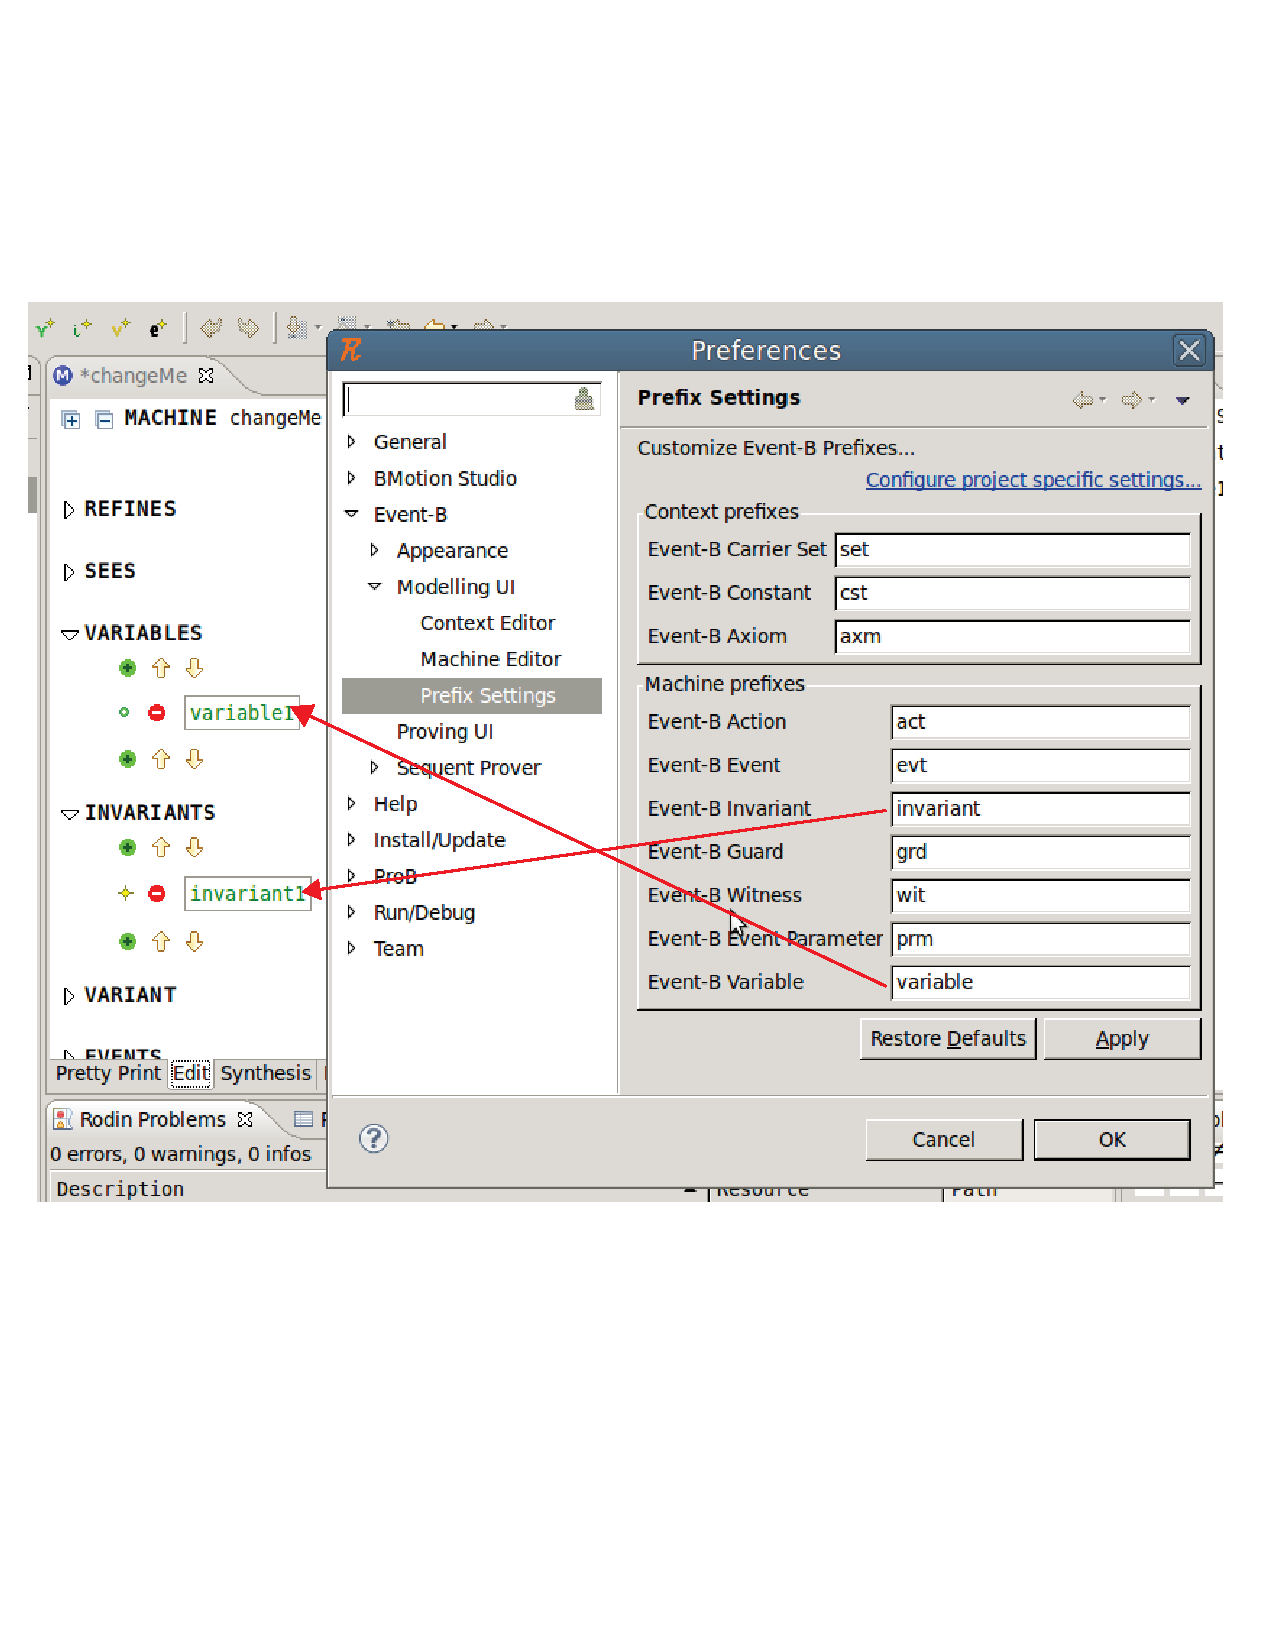
\includegraphics{img/reference/ref_01_preferences1.png}
%	\caption{The Structured Editor}
%	\label{fig_ref_01_preferences1}
%\end{center}
%\end{figure}

The image above shows that modifying prefixes at a workspace scope or project scope, will affect the names used at creation of new Event-B elements. On this image, one can see that the prefix for a variable (resp. invariant) originally set to "var" (resp. "inv") has been replaced by "variable" (resp. "invariant"). New elements are then named using those prefixes.

How to set prefixes

Prefix settings can be accessed through 2 differents ways depending on the scope of their application:

Workspace scope settings

Window > Preferences > Event-B > Modelling UI > Prefix settings, 
    
%\begin{figure}[!h]
%\begin{center}
%	\includegraphics{img/reference/ref_01_preferences2.png}
%	\caption{The Structured Editor}
%	\label{fig_ref_01_preferences2}
%\end{center}
%\end{figure}

or directly via,

    Rename > Customize prefixes... (The rename menu appeared in previous releases as the refactoring menu) 

%\begin{figure}[!h]
%\begin{center}
%	\includegraphics{img/reference/ref_01_preferences3.png}
%	\caption{The Structured Editor}
%	\label{fig_ref_01_preferences3}
%\end{center}
%\end{figure}

Project scope settings

    by right-clicking on a project and then choosing "Properties",
    Menu "Project > Properties",
    or via the Window > Preferences and then click on the link "Configure project specific settings". In this case, one will have to choose the project on which the prefixes should be set up. This is allowed via a specific project selection dialog. After the project selection, a dialog for prefix settings opens for the selected project. 

A dialog (see picture below) appears, where a page handling prefixes settings, allows one user to customize prefixes for a chosen project. One this page, the user can toggle the button "Enable project specific settings".

    If this button is enabled :
        the prefixes used are those which are specified at this project level, 
    If this button is not enabled :
        the prefixes used are those which are defined at a workspace level. 

%\begin{figure}[!h]
%\begin{center}
%	\includegraphics{img/reference/ref_01_preferences4.png}
%	\caption{The Structured Editor}
%	\label{fig_ref_01_preferences4}
%\end{center}
%\end{figure}

Automatic Renaming

    One action is available for Context files.
        Automatic Axiom Labelling : this action will perform alphanumeric renaming on axioms given their order of appearance.
 
%\begin{figure}[!h]
%\begin{center}
%	\includegraphics{img/reference/ref_01_preferences5.png}
%	\caption{The Structured Editor}
%	\label{fig_ref_01_preferences5}
%\end{center}
%\end{figure}

Three actions are available for Machine files.

    Automatic Invariant Labelling : this action will perform alphanumeric renaming on invariants given their order of appearance,
    Automatic Guard Labelling : this action will perform alphanumeric renaming on guards given their order of appearance,
    Automatic Action Labelling : this action will perform alphanumeric renaming on guards given their order of appearance. 

%\begin{figure}[!h]
%\begin{center}
%	\includegraphics{img/reference/ref_01_preferences6.png}
%	\caption{The Structured Editor}
%	\label{fig_ref_01_preferences6}
%\end{center}
%\end{figure}

\subsubsection{Preferences for the automatic tactics}

\marginpar{CONTENT MIGRATED FROM WIKI!}

\paragraph{Introduction}

The purpose is to give more detailed preferences to the user to build his own automated tactics. More precisely, the user should on the one hand have a way to specify which parameters have to be passed to the reasoners, and on the other hand to construct complex proof strategies.

\paragraph{User Documentation}

Here is the documentation about the current implementation of automatic tactics preferences: Auto-tactic \& Post-tactic

\paragraph{Tactic Combinators}

Tactic combinators can be used to construct complex proof strategies.

Historically, one combinator exists since the beginning of auto tactic preferences: the "loop on all pending". It takes one or more tactics and loops them over every pending child, until all tactic fail. Until Rodin 2.3, it is the only combinator in Rodin; it is used on the configurable list of auto and post tactics. Rodin 2.3 pushes configurability forward, by providing several other combinators and auto tactic editors.

The following is a list of combinators present by default.

One may notice the absence of child-specific combinator, i.e applying tactic T1 on first child, T2 on second child, ..., whereas this kind of combinator exists in other provers. The reason is that we are constructing here auto tactics, that is tactics to be attempted in a general context. In provers with child-specific combinators, they are used to make manual proofs, hence needing proof-specific adaptation.

\subparagraph{Composers}

A composer combinator applies its given tactic(s) to the given node. The given node may be open or closed. It succeeds if at least 1 tactic application succeeded. 

\begin{center}
    \begin{tabular}{ | l | l | l | l | p{5cm} |}
    \hline
	Name & Arity & Description & Stops when  \\ \hline
	Sequence & 1..n  & applies given tactics in given order & all tactics have been applied  \\ \hline
	Compose until Success & 1..n  & applies given tactics in given order & a tactic application succeeds \\ \hline
	Compose until failure  & 1..n  & applies given tactics in given order & a tactic application fails \\ \hline
	Loop & 1 & applies given tactic repeatedly & the child tactic application fails \\ \hline
    \end{tabular}
\end{center}

\subparagraph{Selectors}

A selector combinator applies its given tactic to the set of nodes it selects. Selected nodes are computed from the given node. The given node may be open or closed. It succeeds if the tactic application succeeded for at least 1 selected node. 

\begin{center}
    \begin{tabular}{ | l | l | l | p{5cm} |}
    \hline
	Name & Arity & Selects \\ \hline
	On all pending  & 1 & all pending children of the given node (the given node itself if it is open) \\ \hline
    \end{tabular}
\end{center}

\subparagraph{Post Actions}

A post actions applies its given tactic to the given node. The given node must be open (else it fails). Then, it performs a specific treatment, guarded by a trigger condition. 

\begin{center}
    \begin{tabular}{ | l | l | l | l | p{5cm} |}
    \hline
	Name & Arity & Trigger Condition & Post Action \\ \hline
	Attempt & 1 & the given node still has pending children (subtree not closed) & prune proof tree at given node  \\ \hline
    \end{tabular}
\end{center}

\subparagraph{Loop on All pending}

$loopOnAllPending(T_1 \ldots T_n) \;\;\defi\;\; loop(onAllPending(composeUntilSuccess(T_1 \ldots T_n)))  $

\paragraph{Other Ideas}

    timeout: a post action of arity 1 (with duration as input): limits the time allocated for the tactic it is applied to (fails after time has gone out)

    limitDepth: a post action of arity 1 (with depth as input): limits the proof tree depth for the tactic it is applied to (prevents tree from growing beyond a given depth) 

\subsubsection{Proof Skeleton View}

\marginpar{CONTENT MIGRATED FROM WIKI!}

The text field on top of the \textsf{Event-B Explorer} can be used to filter displayed proof obligations. Only POs with a name that contains the input text will appear in the view. We will start an example from the following: 

To browse through a proof, you can use the Proof Skeleton View.

As can be seen in the screen shot above, machine "celebrity\_1" of project "celebrity" is expanded. We find seven proof obligations. Each of them has got a compound name as indicated in the tables below. A green logo situated on the left of the proof obligation name states that it has been proved (an A means it has been proved automatically). If you switch in proving perspective and click on the proof obligation name in the Event-B Explorer, you are transferred into a window where you can handle your proof. We are going to describe it more precisely in subsequent sections.



Purpose

The Proof Skeleton View allows to quickly browse through a proof built either automatically or interactively with the Rodin prover. This view can be used on any proof, independently of the presence of a corresponding proof obligation.

Furthermore, this view allows user to see together proof rules and corresponding sequents.

The Proof Skeleton View
Showing the View

The Proof Skeleton View is available as other views in the Window > Show View > Other > Event-B > Proof Skeleton View menu.

To watch a proof skeleton, simply select a proof obligation or a proof file in the Event-B Explorer.

View Interpretation

Proof skeletons are displayed in a two-part view. On the left-hand side is the tree structure of rules applied in the proof. On the right-hand side stands the sequent on which the currently selected rule is applied. The proof which is displayed is the one stored in the proof file on disk, never the one which is currently edited through the proof control. This can be very handy as it can allow one to see the previous proof of a proof obligation while working on a new proof of it. 

%\begin{figure}[!h]
%\begin{center}
%	\includegraphics{img/reference/ref_01_proofskeletonview1.jpg}
%	\caption{A typical example of machine and context relationship}
%	\label{fig_ref_01_proofskeletonview1}
%\end{center}
%\end{figure}

The tree can be expanded or collapsed by using [+] and [-] buttons on the upper right corner.

Copy/Paste to Proof Tree

The copy/paste feature allows to reuse a stored proof into a new proof. Starting from the following configuration: 

%\begin{figure}[!h]
%\begin{center}
%	\includegraphics{img/reference/ref_01_proofskeletonview2.png}
%	\caption{A typical example of machine and context relationship}
%	\label{fig_ref_01_proofskeletonview2}
%\end{center}
%\end{figure}

where the proof we are working on (top left) is similar to another proof whose skeleton is displayed on bottom left. We can then copy/paste the interesting sub tree from the skeleton to the proof: 

%\begin{figure}[!h]
%\begin{center}
%	\includegraphics{img/reference/ref_01_proofskeletonview3.png}
%	\caption{A typical example of machine and context relationship}
%	\label{fig_ref_01_proofskeletonview3}
%\end{center}
%\end{figure}

%\begin{figure}[!h]
%\begin{center}
%	\includegraphics{img/reference/ref_01_proofskeletonview4.png}
%	\caption{A typical example of machine and context relationship}
%	\label{fig_ref_01_proofskeletonview5}
%\end{center}
%\end{figure}

%\begin{figure}[!h]
%\begin{center}
%	\includegraphics{img/reference/ref_01_proofskeletonview5.png}
%	\caption{A typical example of machine and context relationship}
%	\label{fig_ref_01_proofskeletonview5}
%\end{center}
%\end{figure}

